\subsection{Rozdzielenie tensorów na paczki}
Jednym ze sposobów przyspieszenia czasu uczenia jest podzielenie danych na paczki (ang. batche).
Pozwala nam to na wykonywanie obliczeń na wielu danych jednocześnie. W naszej bibliotece 
wymiarami batcha zawsze będzie: (rozmiar batcha) $x$ (rozmiar alfabetu) $x$ (ilość timestepów). 
Poniżej przedstawiamy batchowanie na przykładzie, dla którego przyjmiemy następujące założenia: 
\begin{itemize}
	\item rozmiar batcha równy 3
	\item liczba timestepów równa 3
	\item liczba autorów równa 4
	\item alfabet $\{a,b,c,d\}$
\end{itemize}

Każdy z autorów ma przyporządkowane nastpujące teksty:
\begin{itemize}
	\item autor 1: ``abacd''
	\item autor 2: ``dbaa''
	\item autor 3: ``cadb''
	\item autor 4: ``cbbcc''
\end{itemize}

Zamieniamy litery na wektory wedle wcześniejszego opisu, gdzie:
\vspace{3mm}
\newline 
$
a =
\begin{bmatrix} 
1, & 0, & 0, & 0
\end{bmatrix} 
$
\vspace{3mm}
\newline
$
b = 
\begin{bmatrix} 
0, & 1, & 0, & 0
\end{bmatrix} 
$
\vspace{3mm}
\newline 
$
c =
\begin{bmatrix} 
0, & 0, & 1, & 0
\end{bmatrix} 
$
\vspace{3mm}
\newline 
$
d =
\begin{bmatrix} 
0, & 0, & 0, & 1
\end{bmatrix} 
$
\vspace{1mm}
\newline 

Wektory umieszczamy w tensorach. Dla każdego autora przewidziany jest osobny tensor. 
Przykładowo dla autora 3 wyglądałby on następująco:
\vspace{3mm}

$
\begin{bmatrix} \begin{bmatrix} 0, & 0, & 1, & 0\end{bmatrix},  & \begin{bmatrix} 1, & 0, & 0, & 0\end{bmatrix}, & \begin{bmatrix} 0, & 0, & 0, & 1\end{bmatrix}, & \begin{bmatrix} 0, & 1, & 0, & 0\end{bmatrix} \end{bmatrix}
$



\begin{wrapfigure}{r}{0.6\textwidth}
\vspace{-4mm}
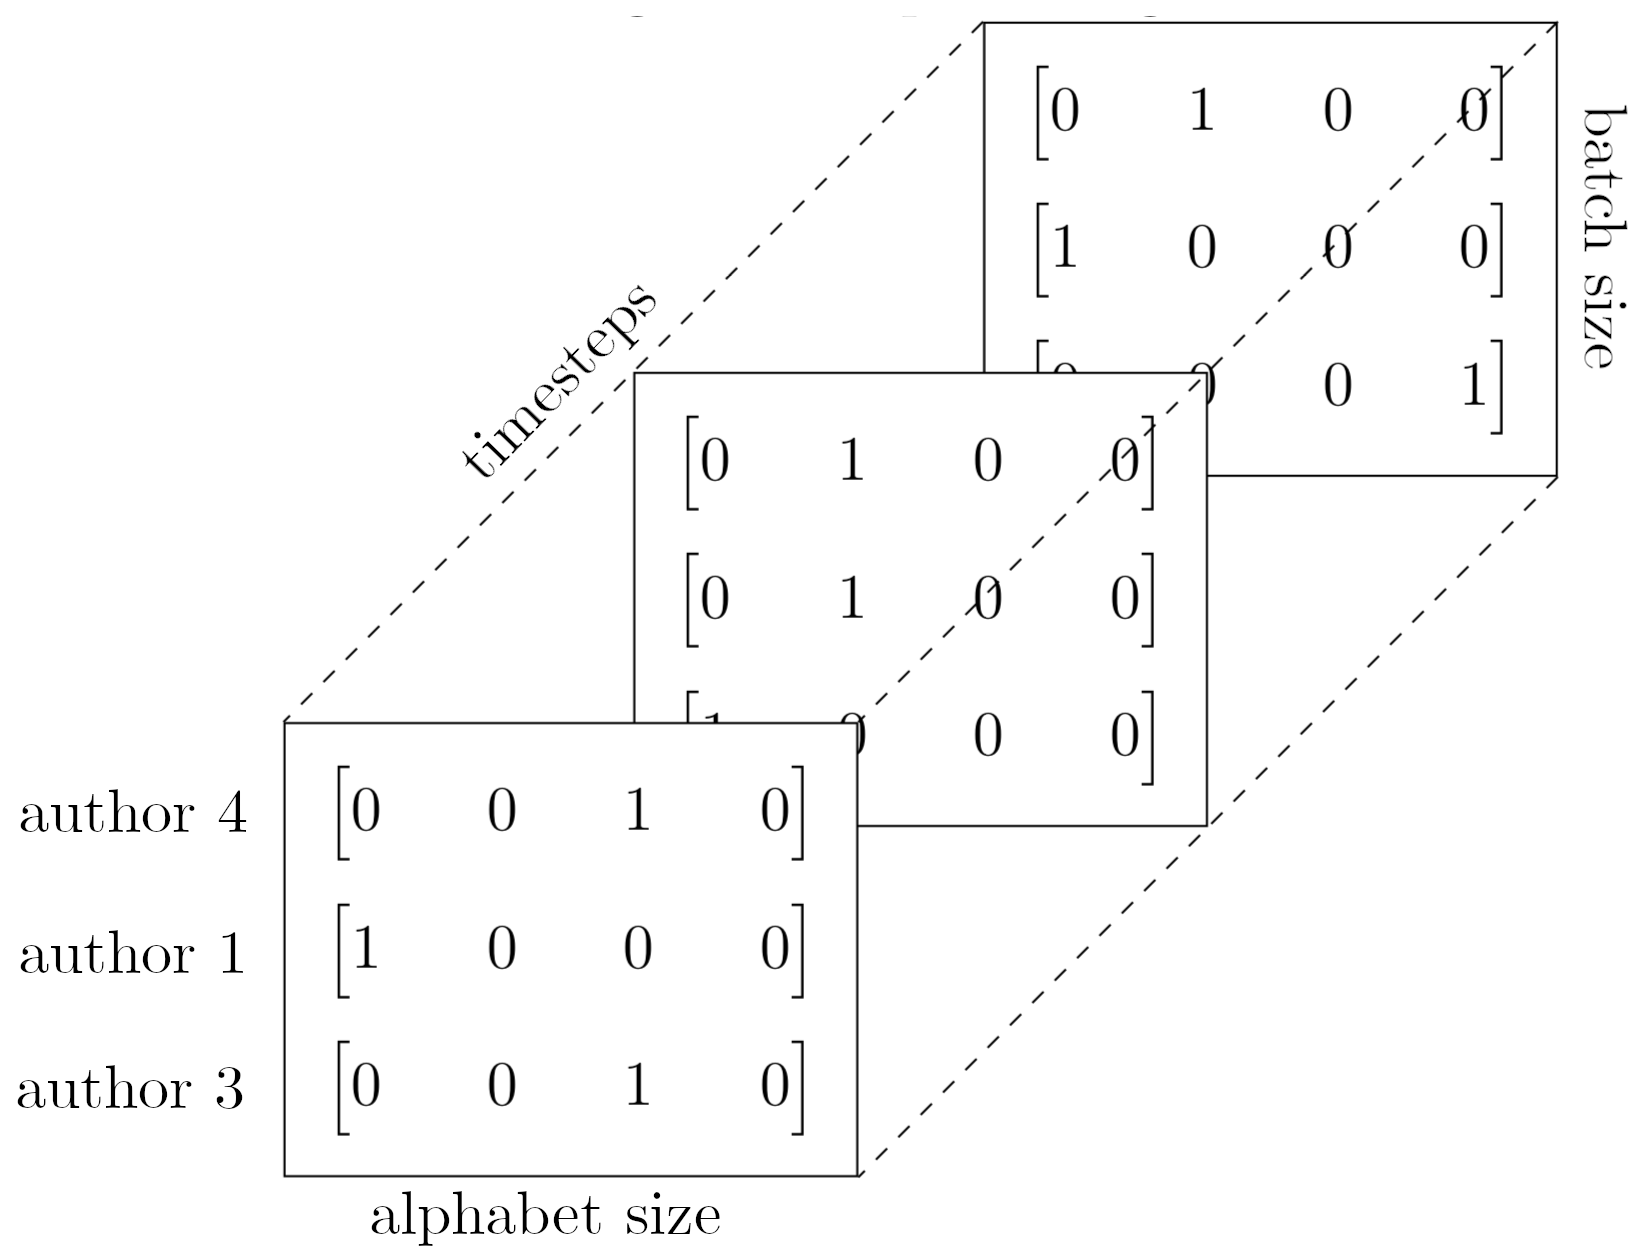
\includegraphics[width=\linewidth]{./images/batch.png}
\caption{Wizualizacja pierwszego batcha}
\label{fig:test2}
\vspace{-4mm}
\end{wrapfigure}
\vspace{4mm}
Następnie ze wszystkich tych tensorów tworzymy batche.
Dla tego przykładu każdy z batchy będzie tensorem o wymiarach 3 x 4 x 3 ((rozmiar batcha) $x$ 
(rozmiar alfabetu) $x$ (ilość timestepów)).
Do każdej takiej paczki będziemy losować autorów oraz ich kolejność. Załóżmy, że do pierwszego batcha
wylosowaliśmy autora 4, 1 oraz 3. Oznacza to, że w pierwszym timestepie w tensorze zawarta będzie 
patrząc ``od góry'': pierwsza litera autora 4, pierwsza litera autora 1 oraz pierwsza litera autora 3.
To ustawienie autorów w tensorach będzie już zawsze zachowane dla wszystkich timestepów w tym batchu. 
A więc dla drugiego timestepu będzie to: druga litera autora 4, druga litera autora 1 oraz druga 
litera autora 3. Dla trzeciego timestepu analogicznie. 

Może się zdarzyć sytuacja, że do batcha wylosowano kilkukrotnie tego samego autora. Na przykład wylosowano
autorów 1 oraz 3, w kolejności: autor pierwszy, następnie znowu autor pierwszy, na końcu autor trzeci.
Dla identycznych założeń jak we wcześniejszym przykładzie w pierwszym batchu w pierwszym timestepie wyglądałoby to
 następująco: pierwsza litera autora 1, następnie pierwsza litera autora 1,
na końcu pierwsza litera autora 3. W drugim timestepie byłoby to:
druga litera autora 1, druga litera autora 1 oraz druga litera autora 3, itd.

Ilość batchy jest zależna od długości tekstów. Są tworzone dopóki nie skończą się znaki w tensorze
któregoś z autorów, dlatego teksty powinny być mniej więcej tej samej długości. Sieć można
wyszkolić dobrze tylko zachowując maksymalnie dużą losowość wystąpień autorów w każdym batchu.
